\documentclass[12pt, titlepage]{article}

\usepackage{fullpage}
\usepackage[round]{natbib}
\usepackage{multirow}
\usepackage{booktabs}
\usepackage{tabularx}
\usepackage{graphicx}
\usepackage{xr}
\usepackage{float}
\usepackage{hyperref}
\hypersetup{
    colorlinks,
    citecolor=blue,
    filecolor=magenta,
    linkcolor=black,
    urlcolor=cyan
}

%% Comments

\usepackage{color}

\newif\ifcomments\commentstrue

\ifcomments
\newcommand{\authornote}[3]{\textcolor{#1}{[#3 ---#2]}}
\newcommand{\todo}[1]{\textcolor{red}{[TODO: #1]}}
\else
\newcommand{\authornote}[3]{}
\newcommand{\todo}[1]{}
\fi

\newcommand{\wss}[1]{\authornote{blue}{SS}{#1}}
\newcommand{\hz}[1]{\authornote{magenta}{Author}{#1}}

\externaldocument{../../SRS/CA}

\newcounter{acnum}
\newcommand{\actheacnum}{AC\theacnum}
\newcommand{\acref}[1]{AC\ref{#1}}

\newcounter{ucnum}
\newcommand{\uctheucnum}{UC\theucnum}
\newcommand{\uref}[1]{UC\ref{#1}}

\newcounter{mnum}
\newcommand{\mthemnum}{M\themnum}
\newcommand{\mref}[1]{M\ref{#1}}

\newcommand{\famname}{LoSMS} % PUT YOUR PROGRAM NAME %HERE

\begin{document}

\title{Module Guide: A Library of Simplex Method Solvers (\famname{}) \wss{Work 
the name of your library into your MG title}\hz{done.}} 
\author{Hanane Zlitni}
\date{November 05, 2018}

\maketitle

\pagenumbering{roman}

\section{Revision History}

\begin{tabularx}{\textwidth}{p{3cm}p{2cm}X}
\toprule {\bf Date} & {\bf Version} & {\bf Notes}\\
\midrule
December 17, 2018 & 2.0 & Final Draft (includes making the document consistent 
with the rest of the deliverables)\\
December 16, 2018 & 1.2 & Applied Dr.~Smith’s Comments\\
December 06, 2018 & 1.1 & Applied Vajiheh Motamer's Comments Posted on GitHub\\
November 05, 2018 & 1.0 & First Draft\\
\bottomrule
\end{tabularx}

~\newpage

\section{Symbols, Abbreviations and Acronyms}

See SRS Documentation at 
\url{https://github.com/hananezlitni/HZ-CAS741-Project/blob/master/docs/SRS/CA.pdf}.
\\

The following are additional symbols, abbreviations or acronyms used in this 
document: \\

\renewcommand{\arraystretch}{1.2}
\begin{tabular}{l l} 
	\toprule		
	\textbf{symbol} & \textbf{description}\\
	\midrule 
	AC & Anticipated Change\\
	UC & Unlikely Change\\
	M & Module\\
	OS & Operating System\\
	DAG & Directed Acyclic Graph\\
	\bottomrule
\end{tabular}\\

\newpage

\tableofcontents

\listoftables

\listoffigures

\newpage

\pagenumbering{arabic}

\section{Introduction}

Decomposing a system into modules is a commonly accepted approach to developing
software.  A module is a work assignment for a programmer or programming
team~\citep{ParnasEtAl1984}.  We advocate a decomposition
based on the principle of information hiding~\citep{Parnas1972a}.  This
principle supports design for change, because the ``secrets'' that each module
hides represent likely future changes.  Design for change is valuable in SC,
where modifications are frequent, especially during initial development as the
solution space is explored.  

Our design follows the rules layed out by \citet{ParnasEtAl1984}, as follows:
\begin{itemize}
\item System details that are likely to change independently should be the
  secrets of separate modules.
\item Each data structure is used in only one module.
\item Any other program that requires information stored in a module's data
  structures must obtain it by calling access programs belonging to that module.
\end{itemize}

After completing the first stage of the design, the Software Requirements
Specification (SRS), the Module Guide (MG) is developed~\citep{ParnasEtAl1984}. The MG
specifies the modular structure of the system and is intended to allow both
designers and maintainers to easily identify the parts of the software.  The
potential readers of this document are as follows:

\begin{itemize}
\item New project members: This document can be a guide for a new project member
  to easily understand the overall structure and quickly find the
  relevant modules they are searching for.
\item Maintainers: The hierarchical structure of the module guide improves the
  maintainers' understanding when they need to make changes to the system. It is
  important for a maintainer to update the relevant sections of the document
  after changes have been made.
\item Designers: Once the module guide has been written, it can be used to
  check for consistency, feasibility and flexibility. Designers can verify the
  system in various ways, such as consistency among modules, feasibility of the
  decomposition, and flexibility of the design.
\end{itemize}

The rest of the document is organized as follows. Section
\ref{SecChange} lists the anticipated and unlikely changes of the software
requirements. Section \ref{SecMH} summarizes the module decomposition that
was constructed according to the likely changes. Section \ref{SecConnection}
specifies the connections between the software requirements and the
modules. Section \ref{SecMD} gives a detailed description of the
modules. Section \ref{SecTM} includes two traceability matrices. One checks
the completeness of the design against the requirements provided in the SRS. The
other shows the relation between anticipated changes and the modules. Section
\ref{SecUse} describes the use relation between modules.

\section{Anticipated and Unlikely Changes} \label{SecChange}

This section lists possible changes to the system. According to the likeliness
of the change, the possible changes are classified into two
categories. Anticipated changes are listed in Section \ref{SecAchange}, and
unlikely changes are listed in Section \ref{SecUchange}.

\subsection{Anticipated Changes} \label{SecAchange}

Anticipated changes are the source of the information that is to be hidden
inside the modules. Ideally, changing one of the anticipated changes will only
require changing the one module that hides the associated decision. The approach
adapted here is called design for
change.

\begin{description}
\item[\refstepcounter{acnum} \actheacnum \label{acHardware}:] The specific
  hardware on which the software is running.
  
\item[\refstepcounter{acnum} \actheacnum \label{acInput}:] The format of the
  initial input data.
  
\item[\refstepcounter{acnum} \actheacnum \label{acInputAssumption}:] The 
assumptions related to the input data discussed in Section \ref{Assumptions} in 
the CA (\cite{losms-ca}).

\item[\refstepcounter{acnum} \actheacnum \label{acInputDataStructure}:] The 
data structure used to store the input data.

\item[\refstepcounter{acnum} \actheacnum \label{acAlgorithm}:] The linear 
programming algorithm used to obtain the optimal solution.

\item[\refstepcounter{acnum} \actheacnum \label{acOutput}:] The format of the 
final output data.
\end{description}

\subsection{Unlikely Changes} \label{SecUchange}

The module design should be as general as possible. However, a general system is
more complex. Sometimes this complexity is not necessary. Fixing some design
decisions at the system architecture stage can simplify the software design. If
these decisions should later need to be changed, then many parts of the design
will potentially need to be modified. Hence, it is not intended that these
decisions will be changed.

\begin{description}
\item[\refstepcounter{ucnum} \uctheucnum \label{ucIO}:] Input/Output devices
  (Input: File and/or Keyboard, Output: File, Memory, and/or Screen).

\item[\refstepcounter{ucnum} \uctheucnum \label{ucObjective}:] The objective of 
the \famname{} library will always be to find and output the optimal 
solution of linear programs along with the values of the decision variables 
given the objective function, linear constraints and the objective function 
goal.
\end{description}

\section{Module Hierarchy} \label{SecMH}

This section provides an overview of the module design. Modules are summarized
in a hierarchy decomposed by secrets in Table \ref{TblMH}. The modules listed
below, which are leaves in the hierarchy tree, are the modules that will
actually be implemented.

\begin{description}
\item [\refstepcounter{mnum} \mthemnum \label{mHH}:] Hardware-Hiding Module
\item [\refstepcounter{mnum} \mthemnum \label{mBH}:] Behaviour-Hiding Module
\item [\refstepcounter{mnum} \mthemnum \label{mSimplex}:] Simplex Method Solver 
Module
\item [\refstepcounter{mnum} \mthemnum \label{mExceptions}:] Exceptions Module
\end{description}

Note that \mref{mHH} is a commonly used module and is already implemented by 
the operating system. Therefore, it will not be reimplemented. Furthermore, for 
the current scope of the project where minimization linear programs are solved 
by converting them to maximization problems, it makes more sense to have one 
simplex method solver module that provides services for solving both types of 
problems. In case of further expansion of the project and the usage of other 
variations of the algorithm to solve minimization problems, it would then make 
more sense to have two separate simplex method modules: one for maximization 
problems and one for minimization problems.

\begin{table}[h!]
\centering
\begin{tabular}{p{0.3\textwidth} p{0.6\textwidth}}
\toprule
\textbf{Level 1} & \textbf{Level 2}\\
\midrule

{Hardware-Hiding Module} & ~ \\
\midrule

{Behaviour-Hiding Module} & ~ \\
\midrule

\multirow{3}{0.3\textwidth}{Software Decision Module}
& Simplex Method Solver\\
& Exceptions\\
\bottomrule

\end{tabular}
\caption{Module Hierarchy}
\label{TblMH}
\end{table}

\section{Connection Between Requirements and Design} \label{SecConnection}

The design of the system is intended to satisfy the requirements developed in
the SRS. In this stage, the system is decomposed into modules. The connection
between requirements and modules is listed in Table \ref{TblRT}.

\section{Module Decomposition} \label{SecMD}

Modules are decomposed according to the principle of ``information hiding''
proposed by \citet{ParnasEtAl1984}. The \emph{Secrets} field in a module
decomposition is a brief statement of the design decision hidden by the
module. The \emph{Services} field specifies \emph{what} the module will do
without documenting \emph{how} to do it. For each module, a suggestion for the
implementing software is given under the \emph{Implemented By} title. If the
entry is \emph{OS}, this means that the module is provided by the operating
system or by standard programming language libraries.  Also indicate if the
module will be implemented specifically for the software.

Only the leaf modules in the
hierarchy have to be implemented. If a dash (\emph{--}) is shown, this means
that the module is not a leaf and will not have to be implemented. Whether or
not this module is implemented depends on the programming language
selected.

\subsection{Hardware Hiding Modules (\mref{mHH})}

\begin{description}
\item[Secrets:]The data structure and algorithm used to implement the virtual
  hardware.
\item[Services:]Serves as a virtual hardware used by the rest of the
  system. This module provides the interface between the hardware and the
  software. So, the system can use it to display outputs or to accept inputs.
\item[Implemented By:] OS
\end{description}

\subsection{Behaviour-Hiding Module (\mref{mBH})}

\begin{description}
\item[Secrets:]The contents of the required behaviours.
\item[Services:]Includes programs that provide externally visible behaviour of
  the system as specified in the software requirements specification (SRS)
  documents. This module serves as a communication layer between the
  hardware-hiding module and the software decision module. The programs in this
  module will need to change if there are changes in the SRS.
\item[Implemented By:] --
\end{description}

\subsection{Software Decision Module}

\begin{description}
\item[Secrets:] The design decision based on mathematical theorems, physical
  facts, or programming considerations. The secrets of this module are
  \emph{not} described in the SRS.
\item[Services:] Includes data structure and algorithms used in the system that
  do not provide direct interaction with the user. 
  % Changes in these modules are more likely to be motivated by a desire to
  % improve performance than by externally imposed changes.
\item[Implemented By:] --
\end{description}

\subsubsection{Simplex Method Solver (\mref{mSimplex})}

\begin{description}
	\item[Secrets:]The structure of the input data, the data structure of the 
	simplex tableau, the simplex algorithm implementation for solving 
	maximization and minimization linear programming problems, the structure of 
	the output data.
	\item[Services:]Receives inputs, checks that they're not empty, throws an 
	error in case of a violation, adds the inputs to a 2D array (simplex 
	tableau), performs the simplex method steps to calculate the solution, 
	outputs the solution to the client.
	\item[Implemented By:] \famname{}
	\item[Justification:] I chose to encapsulate all components of \famname{} 
	in one module because they are so interleaved and highly dependent on one 
	another that separating them caused the modules to have very high coupling.
\end{description}

\subsubsection{Exceptions Module (\mref{mExceptions})}

\begin{description}
	\item[Secrets:]The types of exceptions that the library throws.
	\item[Services:]Catches the exceptions thrown by the simplex solver module 
	and generates the corresponding exception message.
	\item[Implemented By:] \famname{}
\end{description}

\section{Traceability Matrix} \label{SecTM}

This section shows two traceability matrices: between the modules and the
requirements and between the modules and the anticipated changes.

% the table should use mref, the requirements should be named, use something
% like fref
\begin{table}[H]
\centering
\begin{tabular}{p{0.2\textwidth} p{0.6\textwidth}}
\toprule
\textbf{Req.} & \textbf{Modules}\\
\midrule
R\ref{R_Inputs} & \mref{mHH}, \mref{mSimplex}\\
R\ref{R_HandleInputErrors} & \mref{mSimplex}\\
R\ref{R_DisplayErrorMsg} & \mref{mExceptions}\\
R\ref{R_CanonicalForm} & \mref{mSimplex}\\
R\ref{R_Calculate} & \mref{mSimplex}\\
R\ref{R_Output} & \mref{mSimplex}\\
R\ref{R_OutputError} & \mref{mExceptions}\\
\bottomrule
\end{tabular}
\caption{Trace Between Requirements and Modules}
\label{TblRT}
\end{table}

\begin{table}[H]
\centering
\begin{tabular}{p{0.2\textwidth} p{0.6\textwidth}}
\toprule
\textbf{AC} & \textbf{Modules}\\
\midrule
\acref{acHardware} & \mref{mHH}\\
\acref{acInput} & \mref{mSimplex}\\
\acref{acInputAssumption} & \mref{mSimplex}\\
\acref{acInputDataStructure} & \mref{mSimplex}\\
\acref{acAlgorithm} & \mref{mSimplex}\\
\acref{acOutput} & \mref{mSimplex}\\
\bottomrule
\end{tabular}
\caption{Trace Between Anticipated Changes and Modules}
\label{TblACT}
\end{table}

\hz{Is it okay that I didn't include M2 (BH Module) in the tables? Since there 
aren't any BH modules in the hierarchy, I didn't know how to map it with the Rs 
and the ACs} \wss{Yes, this is fine.  The only modules you need to include in the
traceability are the leaf modules.}

\wss{You have two cases where anticipated changes map to more than one module.
  You should explain why this has occurred.  The normal goal is one module, one
  change.  The modules around the input do seem odd.  Could the input module
  have a service (access program) related to conversion?  Do you really need a
  separate module.  Maybe in this case you feel like you have two secrets, but
  if the two secrets always happen together, then module consolidation might
  make sense.  As you write your MIS, it should become clear whether you really
  have two modules.}\hz{the table has been changed to reflect the change in the 
  design.}

\section{Use Hierarchy Between Modules} \label{SecUse}

In this section, the uses hierarchy between modules is
provided. \citet{Parnas1978} said of two programs A and B that A {\em uses} B if
correct execution of B may be necessary for A to complete the task described in
its specification. That is, A {\em uses} B if there exist situations in which
the correct functioning of A depends upon the availability of a correct
implementation of B.  Figure \ref{FigUH} illustrates the use relation between
the modules. It can be seen that the graph is a directed acyclic graph
(DAG). Each level of the hierarchy offers a testable and usable subset of the
system, and modules in the higher level of the hierarchy are essentially simpler
because they use modules from the lower levels.

\begin{figure}[H]
\centering
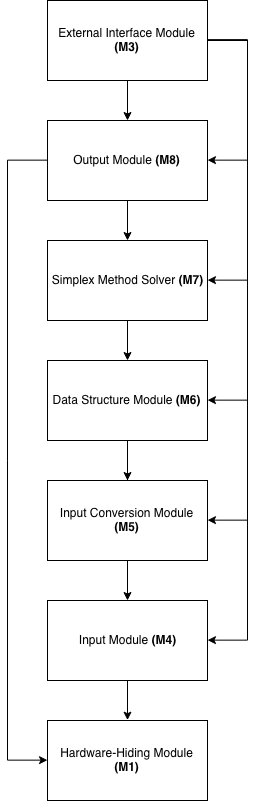
\includegraphics[width=0.3\textwidth]{UsesHierarchy.png}
\caption{Use Hierarchy Among Modules}
\label{FigUH}
\end{figure}

\wss{You indicate that the external interface modules uses the output module
  with two different arrows.  This isn't wrong, but it is confusing.  Does the
  output module really use the simplex method solver?  It seems tome that the
  external interface module would use the simplex solver and then relay the
  results to the output module.  Will the output module actually call the
  simplex solver itself?  I would think that the input module would use the data
  structure module, not the other way around?}\hz{The hierarchy has been 
  changes to reflect the changes in the design.}

\newpage

\bibliographystyle {plainnat}
\bibliography{../../../refs/References}

\end{document}